\section{Experimental Results}%
\label{sec:clgen-eval-results}

We evaluate the effectiveness of our approach on two heterogeneous systems. We first compare the performance of a state-of-the-art predictive model~\cite{Grewe2013} with and without the addition of synthetic benchmarks, then show how the synthetic benchmarks expose weaknesses in the feature design and how these can be addressed to develop a better model. Finally we compare the ability of CLgen to explore the program feature space against a state-of-the-art program generator~\cite{Lidbury2015a}.

\subsection{Performance Evaluation}%
\label{subsec:eval-cgo13}

\begin{figure}
  \centering %
  \subfloat[][AMD Tahiti 7970]{%
    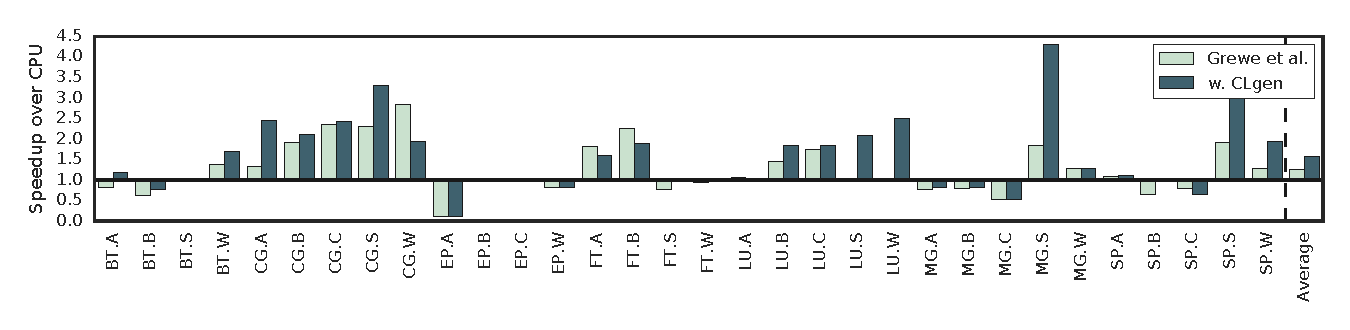
\includegraphics[width=\textwidth]{img/ex1-A}%
    \label{fig:npb-amd}}\\%
  \subfloat[][NVIDIA GTX 970]{%
    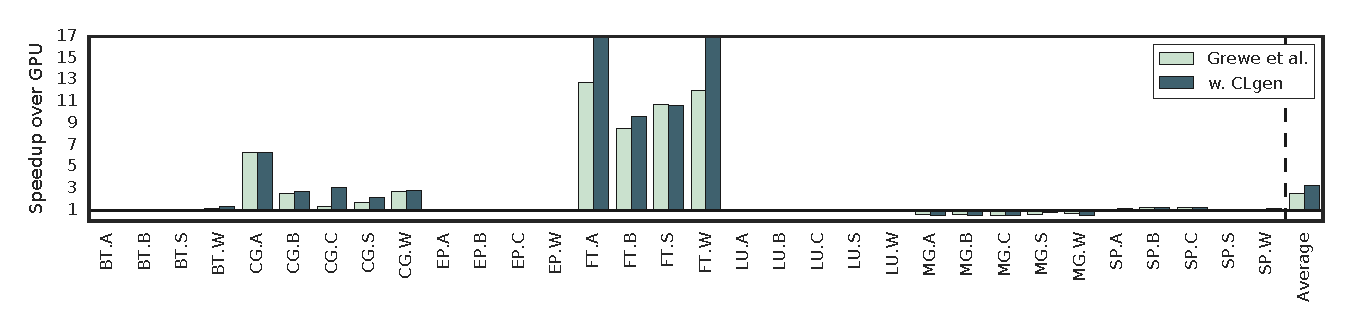
\includegraphics[width=\textwidth]{img/ex1-B}%
    \label{fig:npb-nvidia}}%
  \caption[Speedup of programs with and without synthetic benchmarks]{%
    Speedup of programs using \emph{Grewe et al.\ }predictive model with and without synthetic benchmarks. The predictive model outperforms the best static device mapping by a factor of $1.26\times$ on AMD and $2.50\times$ on NVIDIA. The addition of synthetic benchmarks improves the performance to $1.57\times$ on AMD and $3.26\times$ on NVIDIA.%
  }%
  \label{fig:npb} %
\end{figure}

Figure~\ref{fig:npb} shows speedups of the \emph{Grewe et al.\ }predictive model over the NAS Parallel Benchmark suite with and without the addition of synthesised benchmarks for training. Speedups are calculated relative to the best single-device mapping for each experimental platform, which is CPU-only
for AMD and GPU-only for NVIDIA. The fine grained coverage of the feature space which synthetic benchmarks provide improves performance dramatically for the NAS benchmarks. Across both systems, we achieve an average speedup of $2.42\times$ with the addition of synthetic benchmarks, with prediction improvements over the baseline for 62.5\% of benchmarks on AMD and 53.1\% on NVIDIA.

The strongest performance improvements are on NVIDIA with the \texttt{FT} benchmark which suffers greatly under a single-device mapping. However, the performance on AMD for the same benchmark slightly degrades after adding the synthetic benchmarks, which we address in the next section.

\subsection{Extending the Predictive Model}%
\label{subsec:eval-extended}

\lstinputlisting[%
  label=lst:zero-b,%
  float,%
  caption={%
  	[CLgen program with same features as an AMD benchmark]%
    In the \emph{Grewe et al.\ }feature space this CLgen program is indistinguishable from AMD's Fast Walsh–Hadamard transform benchmark, but has very different runtime behaviour and optimal device mapping. The addition of a branching feature fixes this.%
  },%
  language={[OpenCL]C}
]{lst/zero-b}

Feature designers are bound to select as features only properties which are significant for the sparse benchmarks they test on, which can limit a model's ability to generalise over a wider range of programs. We found this to be the case with the \emph{Grewe et al.\ }model. The addition of automatically generated programs exposed two distinct cases where the model failed to generalise as a result of overspecialising to the NPB suite.

The first case is that \texttt{F3} is sparse on many programs. This is a result of the NPB implementation's heavy exploitation of local memory buffers and the method by which they combined features (we speculate this was a necessary dimensionality reduction in the presence of sparse training programs). To counter this we extended the model to use the raw feature values in addition to the combined features.

The second case is that some of our generated programs had identical feature values as in the benchmark set, but had different \emph{behaviour} (i.e. optimal mappings). Listing~\ref{lst:zero-b} shows one example of a CLgen benchmark which is indistinguishable in the feature space to one the of existing benchmarks --- the Fast Walsh-Hadamard transform --- but with different behaviour. We found this to be caused by the lack of discriminatory features for branching, since the NPB programs are implemented in a manner which aggressively minimised branching. To counter this we extended the predictive model with an additional feature containing a static count of branching operations in a kernel.

Figure~\ref{fig:ex2} shows speedups of our extended model across all seven of the benchmark suites used in Section~\ref{subsec:motivation}. Model performance, even on this tenfold increase of benchmarks, is good. There are three benchmarks on which the model performs poorly: \texttt{MatrixMul}, \texttt{cutcp}, and \texttt{pathfinder}. Each of those programs make heavy use of loops, which we believe the static code features of the model fail to capture. This could be addressed by extracting dynamic instruction counts using profiling, but we considered this beyond the scope of our work. It is not our goal to perfect the predictive model, but to show the performance improvements associated with training on synthetic programs. To this extent, we are successful, achieving average speedups of $3.56\times$ on AMD and $5.04\times$ on NVIDIA across a very large test set.

\begin{figure}
  \centering%
  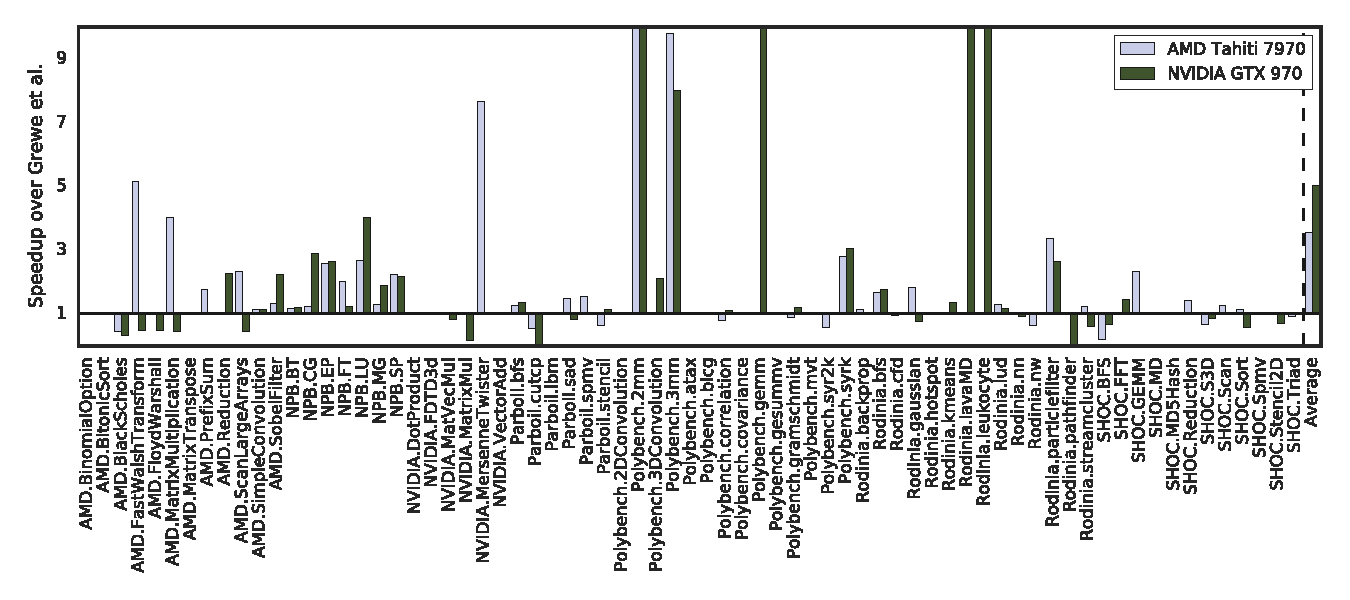
\includegraphics[width=1\textwidth]{img/ex2}%
  \caption[Speedups of predictions using extended model over \emph{Grewe et al.}]{%
    Speedups of predictions using our extended model over \emph{Grewe et al.\ }on both experimental platforms. Synthetic benchmarks and the additional program features outperform the original predictive model by a factor $3.56\times$ on AMD and $5.04\times$ on NVIDIA.%
  }%
  \label{fig:ex2}%
\end{figure}

\subsection{Comparison of Source Features}%
\label{subsec:eval-features}

As demonstrated in Section~\ref{subsec:motivation}, the predictive quality of a model for a given point in the feature space is improved with the addition of observations from neighbouring points. By producing thousands of artificial programs modelled on the structure real OpenCL programs, CLgen is able to consistently and automatically generate programs which are close in the feature space to the benchmarks which we are testing on.

To quantify this effect we use the static code features of Table~\ref{tab:features-raw}, plus the branching feature discussed in the previous subsection, to measure the number of CLgen kernels generated with the same feature values as those of the benchmarks we examined in the previous subsections. We examine only static code features to allow comparison with the GitHub kernels for which we have no automated method to execute them and extract runtime features, and CLSmith generated programs.

Figure~\ref{fig:nn} plots the number of matches as a function of the number of kernels. Out of 10,000 unique CLgen kernels, more than a third have static feature values matching those of the benchmarks, providing on average 14 CLgen kernels for each benchmark. This confirms our original intuition: CLgen kernels, by emulating the way real humans write OpenCL programs, are concentrated in the same area of the feature space as real programs. Moreover, the number of CLgen kernels we generate is unbounded, allowing us to continually refine the exploration of the feature space, while the number of kernels available on GitHub is finite. CLSmith rarely produces code similar to real-world OpenCL programs, with only 0.53\% of the generated kernels have matching feature values with benchmark kernels. We conclude that the unique contribution of CLgen is its ability to generate many thousands of programs \textit{that are appropriate for predictive modelling}.

\begin{figure}
  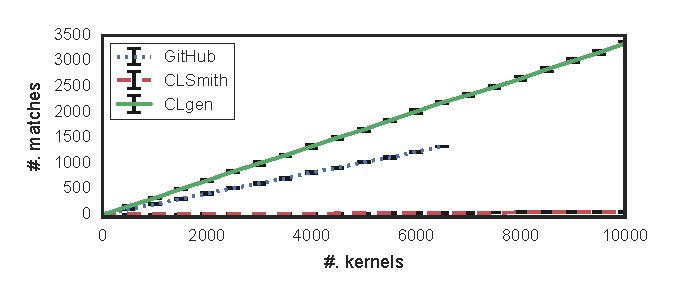
\includegraphics[width=\columnwidth]{img/closeness} %
  \caption[Number of kernels matching benchmark features]{%
    The number of kernels from GitHub, CLSmith, and CLgen with static code features matching the benchmarks. CLgen generates kernels that are closer in the feature space than CLSmith, and can continue to do so long after we have exhausted the extent of the GitHub data set. Error bars show standard deviation of 10 random samplings.%
  }%
  \label{fig:nn}
\end{figure}
